\documentclass[sigconf,nonacm]{acmart}
\settopmatter{printacmref=false,printfolios=true}
\setcopyright{none}
\renewcommand\footnotetextcopyrightpermission[1]{}
\usepackage{amsmath,tabularx,array,enumitem,balance}
\definecolor{CourseBlue}{HTML}{315EFB}
\definecolor{CourseTeal}{HTML}{14877D}
\hypersetup{colorlinks=true,linkcolor=CourseBlue,citecolor=CourseTeal,urlcolor=CourseTeal}
\newcolumntype{Y}{>{\raggedright\arraybackslash}X}
\setlist{leftmargin=*,topsep=3pt,itemsep=2pt}
\newcommand{\CourseNumber}{COMSCI/ECON 206}
\newcommand{\CourseName}{Computational Microeconomics}
\newcommand{\CourseSession}{Autumn 2026 Session 1}
\newcommand{\Instructor}{Luyao Zhang}
\newcommand{\WorkshopSession}{[Your assigned workshop session]}
% Replace these with YOUR fork/project URLs, not the instructor's template.
\newcommand{\GitHubLink}{[Your project GitHub URL]}
\newcommand{\TemplateRepository}{\url{https://github.com/sunshineluyao/ps1-overleaf-template}}
\newcommand{\ColabLink}{[Insert verified Colab URL]}
\newcommand{\DemoLink}{[Insert verified Hugging Face Space URL]}
\newcommand{\coursemeta}{\noindent\textbf{Submission to:} \CourseNumber{} --- \CourseName.\\
\textbf{Course session:} \CourseSession. \textbf{Workshop:} \WorkshopSession.\\
\textbf{Instructor:} \Instructor. \textbf{Assignment:} PS1 research proposal.\par\smallskip}
\title{[A Specific, Researchable Proposal Title]}
\author{[Your Full Name]}
\affiliation{\institution{Duke Kunshan University}\city{Kunshan}\country{China}}
\email{[Your university email]}
\renewcommand{\shortauthors}{[Your name]}

\begin{document}
\begin{teaserfigure}
\captionsetup{skip=8pt}
\centering
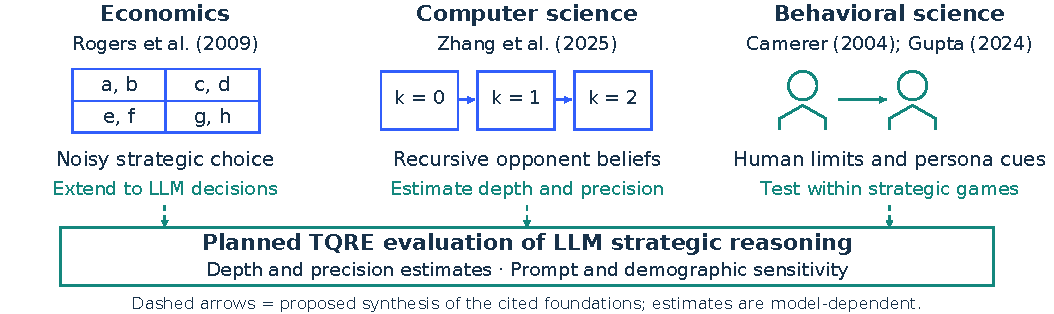
\includegraphics[width=\textwidth]{figures/ps1_teaser.pdf}
\caption{Prospective research design adapted from the class proposal. Economic stochastic choice~\cite{rogers2009}, recursive LLM reasoning~\cite{zhang2025}, human reasoning levels~\cite{camerer2004} and persona audits~\cite{gupta2024} motivate a shared evaluation~\cite{jia2025}. Solid arrows within scenes show conceptual relations; dashed arrows show proposed synthesis. Estimated depth and precision are model-dependent, not direct observations of cognition.}
\Description{Three disciplinary scenes contain a symbolic payoff matrix, successive belief levels, and a comparison of abstract personas. Dashed paths converge on a proposed evaluation of reasoning depth, decision precision and contextual sensitivity. All objects and text are editable in Draw.io.}
\label{fig:teaser}
\end{teaserfigure}
\maketitle\raggedbottom\coursemeta

\noindent\textcolor{CourseTeal}{\textbf{Template and illustrative figure.}} Adapt this class-example diagram and replace prompts with your own proposal. Fork the class repository and import your fork into Overleaf; see README for steps. Keep five numbered sections within two main pages, including metadata, Figure 1, its caption, and artifact links. Author Notes, references, and appendices follow on separate pages.

\section{Three Connected Questions}
\textbf{Economics:} Under quality uncertainty, does a signaling mechanism narrow adverse selection enough to sustain stranger-to-stranger exchange, or does it merely delay market unraveling? \textbf{Computer Science:} Can a lightweight, client-side AI signal make item condition inspectable without a dedicated compute runtime or opaque large-model judgment? \textbf{Behavioral Science:} Does opponent-specific reciprocity emerge among strangers under minimal observability, and how much does an external signal change that emergence? \textbf{Integrated question:} Under a fixed compute and privacy budget, does an AI-assisted trust signal increase completed stranger-to-stranger exchanges on a campus circular-economy platform, and is its effect closer to Akerlof's ``not enough to prevent collapse'' or Leung et al.'s ``enough to bootstrap cooperation''?

\section{Answer to Q1: Economics}
Akerlof's~\cite{akerlof1970} classical result shows that unresolved information asymmetry about quality can depress or collapse a market. A campus exchange platform faces exactly this problem: buyers cannot verify a listed item's true condition before a transaction. Players are the requester (buyer) and the counterpart (seller); actions are list, verify, and trust/decline; payoffs depend on whether the transaction completes and whether the item matches its stated condition. The proposed mechanism narrows, but does not eliminate, this asymmetry through a lightweight verification signal, tested against a no-signal baseline to measure how much of the adverse-selection gap the signal actually closes.

\section{Answer to Q2: Computation}
The mechanism is implemented as a Hugging Face Static Space (\DemoLink), using client-side HTML/CSS/JavaScript only, with no dedicated CPU/GPU runtime, backend, database, or API key. The prototype runs a ten-round trust game under two conditions -- AI-Verified Badge ($p=0.75$) and No Badge/Manual Review ($p=0.45$) -- with seeded logic (seed = 42) so every reported outcome is reproducible. Running the Space's own seeded logic for one ten-round session per condition returned reciprocation in 8 of 10 rounds (80\%) under the Badge condition and 3 of 10 rounds (30\%) under No Badge; these are the artifact's own encoded, illustrative probabilities, not measurements of real campus users. A companion Colab notebook (\ColabLink) reimplements the same probability model in Python to independently verify these round-by-round outcomes.

\clearpage\balance
\section{Answer to Q3: Behavior}
Morozov and Feigel~\cite{morozovfeigel2026} show that strangers can sustain cooperation without full observability through opponent-specific responses, rather than requiring repeated identity tracking. The competing explanation is that any observed cooperation gap reflects only the stated badge probability, not a genuine behavioral response to trust signaling. Discriminating evidence would be a real-user trial where completion rates diverge from the encoded probabilities in a direction opponent-specific reciprocity predicts. Synthetic results from the seeded prototype cannot themselves establish human behavior; a feasible next test is a small live pilot comparing self-reported trust with actual completion under each condition, and a null result -- no behavioral difference beyond the encoded probability -- would change this conclusion.

\section{Advanced Development and Future Directions}
This proposal builds on Akerlof's~\cite{akerlof1970} 1970 Nobel-recognized foundation on information asymmetry in markets, and on the algorithmic-game-theory lineage connecting cooperation, minimal observability, and learning~\cite{leungetal2026}. The enduring human question is how strangers establish trust absent repeated identity or full observability. Today's distinctive environment is a resource-constrained campus platform where verification cannot rely on costly compute or persistent surveillance; current research leaves open how much a lightweight, inspectable signal actually substitutes for full observability, rather than assuming it fully solves adverse selection.

\begin{table}[h]\caption{From laureate foundations to a new interdisciplinary contribution.}
\begin{tabularx}{\columnwidth}{@{}p{1.6cm}Y@{}}\toprule
\textbf{Horizon}&\textbf{Milestone and evidence}\\\midrule
Foundation&Akerlof (1970): adverse selection under quality uncertainty; Leung et al. (2026, AAAI): cooperative learning under minimal observability.\\
PS1&Ten-round trust game (Badge vs.\ No Badge), seeded logic, Colab-verified outputs (8/10 vs.\ 3/10).\\
Next study&Add a live campus pilot comparing self-reported trust with actual completion under each condition.\\
Longer term&Auditable accountability log (Haztrak-style) piloted with the campus sustainability office.\\
2056&A lightweight, resource-aware trust-signaling protocol adopted by resource-constrained institutions.\\\bottomrule
\end{tabularx}\end{table}

\noindent\textbf{Expected 2056 Nobel Prize and Turing Award contribution statement.}
By 2056, I aim to contribute a lightweight, auditable trust-signaling protocol for stranger-to-stranger circular-economy platforms by integrating opponent-specific reciprocity under minimal observability~\cite{morozovfeigel2026} (behavioral advance), signaling mechanisms that counteract adverse selection under quality uncertainty~\cite{akerlof1970} (economic advance), and resource-aware, inspectable AI verification components rather than opaque large-model judgments~\cite{leungetal2026} (computational advance), so that resource-constrained institutions can adopt trust infrastructure without unaccountable AI or unsustainable compute cost. This is an aspiration supported by course-scale milestones, not a prediction of an award.

\subsection*{Open Science Statement}
\textbf{GitHub:} \GitHubLink\\
\textbf{Google Colab:} \ColabLink\par
The repository contains the deployed Space's HTML/CSS/JS source, a Python Colab notebook reimplementing the seeded trust-game logic (seed = 42), and this proposal's LaTeX source. Dependencies are limited to standard Python scientific packages installed in the notebook's setup cell. Shortest reproducible run: open the Colab link and run all cells to regenerate the 8/10 and 3/10 outcomes reported above. Released materials include the full game logic and seeded outputs; validation with real campus users remains a benefit awaiting evaluation, not a released result.

\subsection*{Statement of Contribution to the UN's SDGs}
\textbf{Hugging Face:} \DemoLink\\
Through this open-access interactive trust game, this project aims to support \textbf{SDG Target 12.5}~\cite{sdg12} (substantially reduce waste generation through prevention, reduction, recycling, and reuse) by letting students and staff directly experience how a trust signal changes cooperation incentives in a stranger-to-stranger exchange. Mechanism: an AI-assisted trust signal lowers information asymmetry between strangers, raising the completed exchange/donation rate and diverting items from the waste stream. Observable indicator: the share of initiated exchange/donation requests that reach completion on the campus platform. Distinguishing released from evaluated benefits: the demo itself is released and playable now; its effect on real campus exchange behavior remains to be evaluated.

\subsection*{Submission milestones}
First draft: September 13, 2026, 11:00 P.M. Beijing time (UTC+8). Class review: September 14. Proposed: rebuttal September 16 and revised submission September 20, both at 11:00 P.M. Update Appendix~\ref{app:abstract} with each reflection and revision.

\clearpage\nobalance
\section*{Author Notes}
\subsection*{Acknowledgements}
I thank Prof. Luyao Zhang, Program Chair, and Prof. Ken Rogerson, Program Discussant, of the \emph{2056 Nobel and Turing Laureate Program Launch Workshop}, held at Duke Kunshan University on September 7, 2026. I also thank [full name of teammate 1] and [full name of teammate 2], my teammates in [session number and full session title], and the rest of the COMSCI/ECON 206 Autumn 2026 Session 1 class for their questions and discussion. [Identify a specific contribution you actually used.] I am responsible for the proposal and remaining errors.
\subsection*{Individual contribution}
[State what you personally designed, implemented, wrote, checked, and adapted. Identify shared code or other contributions accurately. Program roles and feedback do not automatically imply coauthorship.]

\bibliographystyle{ACM-Reference-Format}\bibliography{references}
\appendix
\section{Technical details and reproducibility}
[Supply derivations, inputs, package versions, seed where relevant, actual outputs and limitations. Identify repository commit, notebook cells and demo version. Include the fresh-run record.]
\subsection{AI-use disclosure}
AI-Assisted drafting and debugging are permitted after initial independent reasoning. Initial reasoning and handwritten reflection are Human-Only. Record tool/model, date, purpose, significant prompts, accepted or rejected suggestions, human changes and verification. If none, state ``No generative AI was used.'' The human author is responsible for every claim, citation and computation.

\section{Cumulative Intellectual Development}
This proposal develops my Intellectual Statement II through the \emph{2056 Nobel and Turing Laureate Program Launch Workshop}, held on September 7, 2026 at Duke Kunshan University, IB 2050. Program Chair: Prof. Luyao Zhang. Program Discussant: Prof. Ken Rogerson. My session: [number and full title]. My role: [assigned role]. My teammates: [full name 1] and [full name 2]. I acknowledge their contributions and the rest of the class's questions and discussion.

[Trace an earlier claim, a specific dated comment or piece of evidence, and the resulting revision with its intellectual consequence. Do not write only a chronological diary. Retain and revise the 2056 contribution statement.]

Appendix~\ref{app:abstract} contains the structured abstract in the cumulative reflection format. Update its eight rows and preserve the prior version. The Expected 2056 Nobel Prize and Turing Award contribution statement in Section 5 must follow from the foundation, current-era boundary and interdisciplinary milestones.

\section{Field and open-source inspiration}
The \emph{Joint Interdisciplinary Field Trip---Technology, Computation, Culture \& Society in Action} took place on September 4, 2026. Record your actual observations at \textbf{Tencent Shanghai Office} and \textbf{Shanghai Science and Technology Museum}. State attendance accurately.

[Retain one industry photograph and one public-sector photograph from the earlier assignment. Each caption gives exact site, September 4, 2026 visit date, photographer/source, activity or exhibit, and relevance. Distinguish observation from interpretation; connect each setting to an open-source inspiration, subsequent research, and proposed practical value. If you lacked first-hand access, identify an attributed alternative instead of claiming attendance.]

\section{Review response and revision record}
[Retain v1, both peer reviews, author rebuttal, reviewer follow-up and v2. Use the three review themes: strengths to retain, constructive concerns to address, and questions to clarify. Explain your decisions, changed locations and actual verification results. Justify any retained approach or deferred work.]

\clearpage\onecolumn
\section{Structured abstract and cumulative proposal map}\label{app:abstract}
Update this structured abstract with each cumulative reflection. Replace each prompt with a brief, concrete entry and retain earlier versions. The first seven rows summarize the research; the final row records feedback and revision. Detailed optional prompts are in the separate Scaffolding Companion.
\par\medskip
\begin{table}[H]
\caption{Appendix E structured abstract template; retain the eight-row proposal structure.}
\label{tab:abstract-map}
\renewcommand{\arraystretch}{1.18}
\begin{tabularx}{\textwidth}{@{}p{0.27\textwidth}Y@{}}
\toprule
\textbf{Proposal element} & \textbf{Current statement / change} \\
\midrule
Background & State the strategic setting, established knowledge and unresolved issue. Cite the key foundation. \\
Motivation and application & Explain why the issue matters now, the application scenario, affected people and the need the project addresses. \\
Three connected questions & State one economics question, one computer-science question and one behavioral-science question. End with the integrated question that requires all three. \\
Method and model assumptions & Specify players, actions or strategies, incentives, timing and information; then the model, baseline, computation and evidence needed. \\
Results or expected results & State what was actually obtained and label its evidence type. Separately state expected results, the test and what finding would challenge the claim. \\
Intellectual merits & Explain what is learned beyond the cited foundation and why integrating the three disciplines changes the answer. \\
Practical impacts & Identify private- and public-sector value. Explain the open-access learning tool's intended contribution to SDG 4 and how its usefulness could be assessed. \\
Feedback received and revision made & Name the dated feedback source, earlier claim, actual revision and intellectual consequence. Preserve prior versions; state accurately if feedback is pending. \\
\bottomrule
\end{tabularx}
\end{table}
\noindent Keep field observations, photographs, literature notes, open-source inspirations and AI-use disclosure in the supporting sections. Distinguish observation, interpretation and proposed future evidence. The Open Science Statement groups GitHub and Colab; the Statement of Contribution to the UN's SDGs groups the Hugging Face learning tool.


\end{document}
